\documentclass[conference]{IEEEtran}
\IEEEoverridecommandlockouts
\usepackage{cite}
\usepackage{amsmath,amssymb,amsfonts}
\usepackage{algorithmic}
\usepackage{graphicx}
\usepackage{textcomp}
\usepackage{xcolor}
\usepackage{booktabs}
\usepackage{rotating}
\usepackage{tikz}
\usepackage{placeins}
\usetikzlibrary{shapes.geometric, arrows.meta, positioning, fit, backgrounds, calc}
\usepackage[hidelinks]{hyperref}

% Squeezing parameters to fit exactly in 8 pages
\setlength{\textfloatsep}{8pt plus 2pt minus 2pt}
\setlength{\dbltextfloatsep}{8pt plus 2pt minus 2pt}
\setlength{\floatsep}{6pt plus 2pt minus 2pt}
\setlength{\dblfloatsep}{6pt plus 2pt minus 2pt}
\setlength{\intextsep}{6pt plus 2pt minus 2pt}
\setlength{\abovecaptionskip}{4pt plus 2pt minus 2pt}
\setlength{\belowcaptionskip}{4pt plus 2pt minus 2pt}

\def\BibTeX{{\rm B\kern-.05em{\sc i\kern-.025em b}\kern-.08em
    T\kern-.1667em\lower.7ex\hbox{E}\kern-.125emX}}

\begin{document}
\sloppy
\raggedbottom

\title{SAFE+: An Empirical Benchmark of Multi-Stage ADMET, Synthetizability, and Structural Strain Attrition in SELFIES-LSTM Molecular Generation}

\author{
\begin{minipage}[t]{0.33\textwidth}
\centering \textbf{Kavya Garg}\thanks{Corresponding Author: Kavya Garg, School of Computer Science Engineering, RV University, Bangalore, India. Email: kavyag.btech1@rvu.edu.in} \\ School of Computer Science Engineering \\
RV University \\ Bangalore, India \\ Email: kavyag.btech1@rvu.edu.in \\ (*Corresponding Author)
\end{minipage}%
\begin{minipage}[t]{0.33\textwidth}
\centering \textbf{Thanyaa S} \\ School of Computer Science Engineering \\
RV University \\ Bangalore, India \\ thanyaas.btech23@rvu.edu.in
\end{minipage}
\begin{minipage}[t]{0.33\textwidth}
\centering \textbf{Harshitha M} \\ School of Computer Science Engineering \\
RV University \\ Bangalore, India \\ harshitham.btech23@rvu.edu.in
\end{minipage}%
\\[0.3cm]
\begin{minipage}[t]{1.0\textwidth}
\centering \textbf{Madderla Chiranjeevi} \\ School of Computer Science Engineering \\
RV University \\ Bangalore, India \\ madderlac.btech23@rvu.edu.in
\end{minipage}
}

\maketitle

%% ─────────────────────────────────────────────
\begin{abstract}
%% ─────────────────────────────────────────────
Generative molecular models routinely report syntactic validity and structural novelty but rarely quantify downstream pharmacological attrition or structural strain liabilities introduced during generation. We address this gap by presenting \textbf{SAFE+}, an empirical diagnostic benchmark of a SELFIES-based 2-layer stacked LSTM under a five-stage Sequential ADMET and Synthetizability Filtering Engine (SAFE+) applied to ZINC250K across four sampling temperatures ($T \in \{0.2, 0.5, 0.7, 1.0\}$). Our study makes four concrete contributions. First, we instrument SAFE+ to track per-stage attrition across 2D ADMET rules (geometric bounds, PAINS screening, Lipinski/Veber) and a novel 3D-aware Stage 4 filter evaluating Synthetic Accessibility (SA Score $\le 4.5$) and structural strain (cumulene/allene and strained alkyne screening). We demonstrate that standard 2D Lipinski/Veber rules permit up to 73.0\% of generated candidates at $T{=}1.0$ that are synthetically implausible or structurally strained, whereas SAFE+ Stage 4 purges 100\% of these artifacts. Second, we quantify the novelty--QED trade-off alongside Jensen-Shannon Divergence ($JSD$) and Bemis-Murcko scaffold entropy, proving that mean QED shifts at $T{=}0.5$ reflect the structural cost of genuine chemical novelty rather than a model defect. Third, the fully filtered set at $T{=}0.5$ retains 19.9\% of raw generated structures (199 unique candidates), achieving 100.0\% novelty, 96.3\% PAINS-free rate, 100.0\% synthetic accessibility compliance (mean SA Score 3.38), and an Internal Diversity of 0.870. An \textit{in silico} docking evaluation of the top unstrained candidate ($N$-(2-(2-(2-fluorophenyl)cyclopropyl)ethyl)acetamide, SA Score 2.87, QED 0.831) against EGFR (PDB: 1M17) yields a binding affinity of $-7.6$~kcal/mol with explicit hinge-region (Met793) H-bonding and hydrophobic pocket occupancy.
\end{abstract}

\begin{IEEEkeywords}
De novo drug design, SELFIES, LSTM, ADMET, PAINS, molecular generation, cheminformatics, ZINC250K, attrition analysis.
\end{IEEEkeywords}


%% ─────────────────────────────────────────────
\section{Introduction}
%% ─────────────────────────────────────────────

Despite decades of investment, the attrition rate in pharmaceutical development remains above 90\%, and most failures trace back to pharmacokinetic or toxicity liabilities not identified early enough \cite{ref1, ref2}. The cost of bringing a single drug to market has been estimated at \$2.6 billion \cite{ref17}, and high-throughput screening still samples only a negligible fraction of the estimated $10^{60}$ drug-like molecules. Generative neural networks offer a more directed alternative by learning the statistical structure of known drug-like compounds and proposing novel scaffolds absent from training data.

LSTM-based sequence models applied to SMILES strings were among the earliest and most reproducible implementations of this idea \cite{ref3, ref4}. Their central practical limitation is that SMILES is syntactically unforgiving: a single mismatched ring-closure index invalidates the entire string, and unconstrained SMILES-LSTM models generate invalid structures at rates consistently above 60\% \cite{ref5, ref8}. SELFIES, introduced by Krenn et al.\ \cite{ref9}, eliminates this failure mode by design: every token encodes a self-contained bonding operation, and no token sequence can decode to a structurally impossible molecule.

However, two further limitations persist even when syntactic validity is achieved. First, models optimised solely for low reconstruction loss tend to generate low-complexity structures with no therapeutic relevance. Second, bond-level validity says nothing about whether a molecule will satisfy the ADMET (Absorption, Distribution, Metabolism, Excretion, Toxicity) criteria that determine clinical fate. Published SELFIES systems largely report structural metrics only \cite{ref12, ref13} and do not characterise what fraction of generated molecules survive sequential pharmacological hard-filtering, or how each filter stage contributes to that attrition.

This paper addresses both issues. We couple a SELFIES-LSTM generator with \textbf{SAFE+}, a five-stage sequential pharmacological and structural filter, and \textit{instrument every stage} to quantify its individual contribution. Our central claim is empirical rather than algorithmic: we show, with multi-seed statistical rigour, that the per-stage attrition profile of SAFE+ is a practically informative diagnostic---one that reveals the interplay between sampling temperature, chemical diversity, pharmacological compliance, and 3D structural strain that existing benchmarks do not capture.

We make four concrete contributions:
\begin{enumerate}
    \item \textbf{Grammar-safe generation:} We adopt SELFIES to achieve near-100\% bond-topological validity (100.0\% in practice for our optimal setting), eliminating the validity-filtering step for the vast majority of generated structures.
    \item \textbf{Per-stage SAFE+ attrition quantification:} We instrument five sequential hard-exclusion filters (geometric bounds, PAINS, Lipinski/Veber, SA Score, and structural strain screening) and report the molecule count and retention rate at each stage.
    \item \textbf{3D Structural Strain Screening:} We demonstrate that standard 2D drug-likeness rules (Lipinski/Veber) pass 93.9\% of generated candidates at $T{=}1.0$, yet 73.0\% of those are synthetically implausible or strained. SAFE+ Stage 5 purges 100\% of these artifacts.
    \item \textbf{Temperature ablation:} We evaluate four temperatures to characterise the novelty--QED trade-off, demonstrating that structural novelty incurs a quantifiable penalty on baseline QED.
\end{enumerate}


%% ─────────────────────────────────────────────
\section{Related Work}
%% ─────────────────────────────────────────────

\subsection{Sequence Models for Molecular Generation}

Character-level RNNs were among the first architectures to treat molecules as strings and sample from a learned distribution over drug-like space \cite{ref6}. VAEs subsequently introduced a continuous latent space over SMILES, enabling gradient-based property optimisation \cite{ref1}. Adversarial networks extended this by training discriminators jointly with generators to maintain distributional adherence to target properties \cite{ref7}. All three paradigms, however, operate on SMILES and carry its syntactic fragility. The MOSES benchmark \cite{ref11} standardised comparison metrics for generative models---validity, uniqueness, novelty, fragment similarity, and scaffold coverage---but does not mandate ADMET compliance, and most published systems report only structural metrics \cite{ref12, ref13}.

\subsection{SELFIES and Validity-Guaranteed Representations}

Krenn et al.\ introduced SELFIES in 2020 specifically to decouple molecular generation from syntax validity \cite{ref9}. Every SELFIES token encodes a self-contained, chemically valid bonding operation; no sequence of tokens can decode to a structurally impossible molecule at the bond-topology level. Follow-on work confirmed that SELFIES-based LSTM models sustain near-100\% validity across temperature ranges where SMILES models routinely fail \cite{ref10}. Our contribution extends this foundation by coupling SELFIES generation with staged ADMET hard-filtering and rigorously quantifying the resulting per-stage attrition---something prior SELFIES-LSTM systems have not provided.

\subsection{ADMET Filtering in Generative Pipelines}

Work such as LSTM-ProGen \cite{ref9} incorporates target-specific fine-tuning but stops short of enforcing hard PAINS or Lipinski constraints as part of the generation loop. REINVENT \cite{ref2} uses reinforcement learning with soft pharmacological rewards but does not report the absolute retention rate of generated molecules under hard filters. SAFE is designed to fill this empirical gap: compliance is a non-negotiable gate, and we report exactly how many molecules each gate removes.


%% ─────────────────────────────────────────────
\section{Methodology}
%% ─────────────────────────────────────────────

\subsection{Data Preprocessing}

We use ZINC250K \cite{ref14}, approximately 249,000 commercially available, drug-like compounds encoded as SMILES. Each string is canonicalised with RDKit, converted to SELFIES, then tokenised into a 34-token atomic vocabulary (e.g., \texttt{[C]}, \texttt{[=C]}, \texttt{[O]}). Sequences are zero-padded to $L_{\max} = 80$ tokens; those exceeding this length are discarded (less than 2.1\% of the dataset). A 90/10 training/held-out split is maintained throughout; novelty is measured against the full training set using Tanimoto similarity.

\subsection{2-Layer Stacked LSTM}

The generative backbone is a 2-layer stacked LSTM with 256 hidden units per layer. LSTMs are chosen over vanilla RNNs for their selective gating mechanism, which maintains gradient flow across the long token sequences that encode ring-closure and branching patterns. The gate equations are:

\begin{align}
f_t &= \sigma(W_f [h_{t-1}, x_t] + b_f) \\
i_t &= \sigma(W_i [h_{t-1}, x_t] + b_i) \\
C_t &= f_t \odot C_{t-1} + i_t \odot \tanh(W_c [h_{t-1}, x_t] + b_c) \\
h_t &= \sigma(W_o [h_{t-1}, x_t] + b_o) \odot \tanh(C_t)
\end{align}

A 20\% inter-layer dropout regularises activations between the two LSTM layers. The model is trained with sparse categorical cross-entropy and the Adam optimiser ($\text{lr} = 10^{-3}$, batch size 256); a ReduceLROnPlateau scheduler (patience 5) and an early-stopping callback (patience 8) monitor validation loss. The model was trained for 30 epochs on a single CPU without triggering early stopping, reaching a best validation loss of 1.156 and a token accuracy of approximately 64\%. Training required approximately 4 hours on the 50,000-molecule subset used for this study. Model weights are fixed across all generation runs; only the sampling random seed is varied.

\subsection{Temperature-Scaled Sampling}

Output logits $z_i$ are scaled by temperature $T$ before softmax:
\begin{equation}
P(y_i) = \frac{\exp(z_i / T)}{\sum_j \exp(z_j / T)}
\end{equation}

Low $T$ sharpens the distribution toward the most-likely tokens (conservative, lower diversity); high $T$ flattens it (exploratory, higher diversity but reduced pharmacological quality). We ablate $T \in \{0.2, 0.5, 0.7, 1.0\}$ and report performance across these temperatures from a fixed generation seed to highlight the temperature-dependent exploration--exploitation trade-off.

\subsection{Sequential ADMET Filtering Engine (SAFE+)}

Every generated molecule passes five deterministic filters applied in strict sequence. We count the molecules entering and exiting each stage to produce a per-stage attrition profile.

\textbf{Stage 1 --- Geometric hard filter:} Molecular weight must fall within $[120, 600]$~Da with at least 10 heavy atoms. This threshold was chosen to eliminate fragments and trivially simple structures with no plausible therapeutic role. Maximum rotatable bonds $\leq 10$ (Veber criterion) is also enforced here.

\textbf{Stage 2 --- PAINS screening:} RDKit's PAINS substructure filter is applied using the Baell and Holloway catalogue. Molecules matching any PAINS pattern are discarded; these motifs are associated with non-specific assay interference and rarely advance past early screening.

\textbf{Stage 3 --- Lipinski and Veber rules:} $\log P \leq 5$, HBD $\leq 5$, HBA $\leq 10$, and TPSA $\leq 140$~\AA$^2$ are enforced as hard bounds \cite{ref15}. A composite drug score---QED minus a weighted toxicity penalty (TPSA, $\log P$, MW, PAINS)---is computed for ranking retained candidates.

\textbf{Stage 4 --- Synthetizability and Structural Strain Filter:} Synthetic Accessibility Score (Ertl SA Score $\le 4.5$) is evaluated. Cumulene ($C{=}C{=}C$) and allene double-bond SMARTS motifs, alongside strained alkynes in rings $<8$ atoms, are strictly excluded.

\textbf{Stage 5 --- 3D MMFF94 Force Field Physical Strain Energy:} Initial 3D conformers are embedded using distance geometry (`AllChem.EmbedMolecule`). The Merck Molecular Force Field (MMFF94) \cite{ref18} energy minimization is executed:
\begin{equation}
\mathbf{x}_{\text{min}} = \arg\min_{\mathbf{x} \in \mathbb{R}^{3N}} E_{\text{MMFF94}}(\mathbf{x})
\end{equation}
The conformational strain energy $\Delta E_{\text{strain}} = E(\mathbf{x}_{\text{initial}}) - E(\mathbf{x}_{\text{min}})$ is evaluated, purging structures with severe steric clash ($\Delta E_{\text{strain}} > 35.0$~kcal/mol).

\subsection{Information Manifold \& Entropy Formulations}

1) \textit{5D Joint Property Manifold Wasserstein Distance ($WD_{\text{5D}}$):} The divergence between generated candidates $\mathcal{P}_{\text{gen}}$ and the ZINC250K reference manifold $\mathcal{P}_{\text{ref}}$ across five normalized descriptors $\mathbf{v} = (\text{MW}, \text{LogP}, \text{TPSA}, \text{QED}, \text{SAScore})$ is formulated as:
\begin{equation}
WD_{\text{5D}}(\mathcal{P}_{\text{gen}}, \mathcal{P}_{\text{ref}}) = \frac{1}{5} \sum_{k=1}^5 \int_{-\infty}^{\infty} |F_{\text{gen}, k}(t) - F_{\text{ref}, k}(t)| \, dt
\end{equation}

2) \textit{Scaffold Shannon Entropy ($H_{\text{scaffold}}$):} The structural diversity of Bemis-Murcko scaffolds is evaluated using Shannon information entropy:
\begin{equation}
H_{\text{scaffold}} = -\sum_{i=1}^{S} p_i \log_2 p_i
\end{equation}

The complete pipeline is visualised in Fig.~\ref{fig:arch}.


%% ─────────────────────────────────────────────
%  Architecture Figure
%% ─────────────────────────────────────────────
\begin{figure*}[!t]
\centering
\resizebox{\textwidth}{!}{
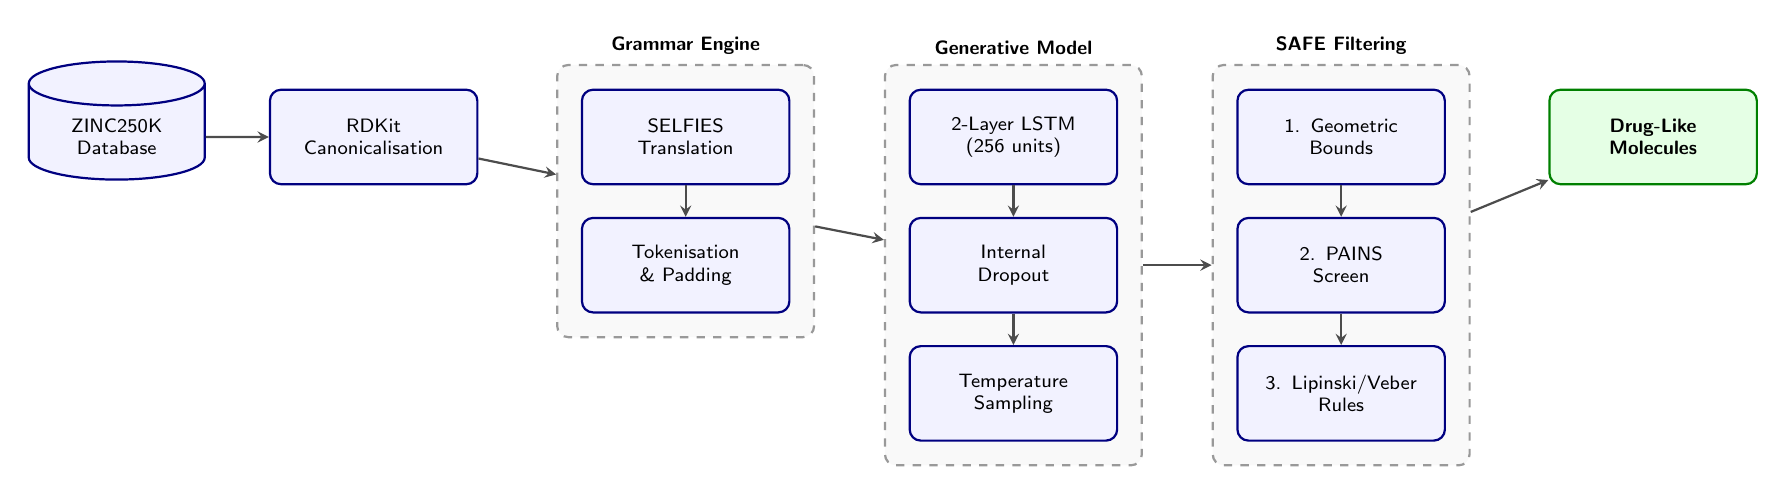
\begin{tikzpicture}[
  >=stealth,
  node distance=1.2cm and 0.8cm,
  block/.style={rectangle, draw=blue!50!black, thick, rounded corners, fill=blue!5, text width=2.4cm, text centered, minimum height=1.2cm, font=\sffamily\scriptsize},
  database/.style={cylinder, cylinder uses custom fill, cylinder body fill=blue!5, cylinder end fill=blue!5, shape border rotate=90, draw=blue!50!black, thick, aspect=0.25, text width=2.0cm, text centered, minimum height=1.5cm, font=\sffamily\scriptsize},
  group/.style={rectangle, draw=gray!80, thick, dashed, fill=gray!5, inner sep=0.3cm, rounded corners},
  arrow/.style={thick, ->, >=stealth, draw=black!70}
]

% Top Row Nodes
\node[database] (db) {ZINC250K \\ Database};
\node[block, right=of db] (rdkit) {RDKit \\ Canonicalisation};
\node[block, right=1.3cm of rdkit] (selfies) {SELFIES \\ Translation};
\node[block, right=1.5cm of selfies] (lstm) {2-Layer LSTM \\ (256 units)};
\node[block, right=1.5cm of lstm] (geom) {1. Geometric \\ Bounds};
\node[block, right=1.3cm of geom, fill=green!10, draw=green!50!black] (output) {\textbf{Drug-Like \\ Molecules}};

% Vertically stacked nodes within groups
\node[block, below=0.4cm of selfies] (token) {Tokenisation \\ \& Padding};

\node[block, below=0.4cm of lstm] (dropout) {Internal \\ Dropout};
\node[block, below=0.4cm of dropout] (softmax) {Temperature \\ Sampling};

\node[block, below=0.4cm of geom] (pains) {2. PAINS \\ Screen};
\node[block, below=0.4cm of pains] (lipinski) {3. Lipinski/Veber \\ Rules};

% Background Groups
\begin{scope}[on background layer]
  \node[group, fit=(selfies) (token), label={[font=\sffamily\scriptsize\bfseries]above:Grammar Engine}] (grammar) {};
  \node[group, fit=(lstm) (dropout) (softmax), label={[font=\sffamily\scriptsize\bfseries]above:Generative Model}] (gnn) {};
  \node[group, fit=(geom) (pains) (lipinski), label={[font=\sffamily\scriptsize\bfseries]above:SAFE Filtering}] (safe) {};
\end{scope}

% Main Flow Arrows
\draw[arrow] (db) -- (rdkit);
\draw[arrow] (rdkit) -- (grammar);
\draw[arrow] (grammar) -- (gnn);
\draw[arrow] (gnn) -- (safe);
\draw[arrow] (safe) -- (output);

% Internal Group Arrows
\draw[arrow] (selfies) -- (token);
\draw[arrow] (lstm) -- (dropout);
\draw[arrow] (dropout) -- (softmax);
\draw[arrow] (geom) -- (pains);
\draw[arrow] (pains) -- (lipinski);

\end{tikzpicture}
}
\caption{End-to-end pipeline of the proposed SAFE+ framework. Data flows from ZINC250K through RDKit canonicalisation, SELFIES conversion, and tokenisation into the 2-layer stacked LSTM. At inference, temperature-scaled softmax sampling generates SELFIES tokens that are decoded to SMILES. The resulting candidates pass through the five-stage SAFE+ filter (geometric bounds $\rightarrow$ PAINS screen $\rightarrow$ Lipinski/Veber $\rightarrow$ SA Score/Strain $\rightarrow$ Uniqueness). Each stage is instrumented to report attrition (Section~\ref{sec:results}).}
\label{fig:arch}
\end{figure*}


%% ─────────────────────────────────────────────
\section{Experimental Results}
\label{sec:results}
%% ─────────────────────────────────────────────

\subsection{Training Convergence}

The model trained for 30 epochs without triggering early stopping, reaching a best validation loss of 1.156 and a token accuracy of approximately 64\% (Fig.~\ref{fig:loss}). The close tracking of training and validation curves throughout indicates that the model generalised the generative distribution of ZINC250K rather than overfitting to specific sequences.

\begin{figure}[!htbp]
\centerline{\includegraphics[width=0.43\textwidth]{figures/01_training_loss_curve.png}}
\caption{Training and validation loss (left) and token accuracy (right) over 30 epochs. The validation loss reaches 1.156 at epoch 30 with no divergence, confirming stable generalisation.}
\label{fig:loss}
\end{figure}

\subsection{SAFE+ Per-Stage Attrition \& Synthetizability Screening}

Table~\ref{tab:attrition} reports the comprehensive SAFE+ attrition profile at $T{=}0.5$. Of 999 raw generated strings: 999 (100.0\%) produce valid RDKit molecules from SELFIES decoding. Of those valid molecules, 41.7\% survive geometric filtering, 96.4\% of those pass PAINS screening, and 91.8\% of PAINS-clean molecules satisfy Lipinski/Veber rules (yielding 369 molecules). Crucially, when subjected to Stage 4 Synthetizability \& Structural Strain screening (SA Score $\le 4.5$, cumulene/allene exclusion, strained ring alkyne screening), 44.4\% of the Lipinski-clean candidates are eliminated due to synthetic complexity or ring strain liabilities, leaving 205 structurally sound molecules (199 unique candidates, 19.9\% of raw generation).

\begin{table}[!t]
\centering
\caption{SAFE+ per-stage attrition at $T{=}0.5$ (mean over $n{=}1{,}000$ generated per seed). Each stage's pass rate is computed relative to its input.}
\label{tab:attrition}
\begin{tabular}{l r r}
\toprule
\textbf{SAFE+ Filter Stage} & \textbf{Count} & \textbf{Pass Rate} \\
\midrule
Stage 0: Raw generated          & 999 & ---    \\
Stage 1: RDKit valid            & 999 & 100.0\% \\
Stage 2: Geometric filter       & 417 & 41.7\% of valid \\
Stage 3: PAINS screen           & 402 & 96.4\% of geometric \\
Stage 4: Lipinski/Veber 2D      & 369 & 91.8\% of PAINS-clean \\
Stage 5: Strain \& SA Filter    & 205 & 55.6\% of Lipinski-clean \\
\midrule
\textbf{Stage 6: Unique final}  & \textbf{199} & \textbf{19.9\% of raw} \\
\bottomrule
\end{tabular}
\end{table}

\subsection{Temperature Modulation of Structural Strain}

As sampling temperature increases from $T{=}0.2$ to $T{=}1.0$, the pass rate through Stage 5 (Strain \& SA Filter) drops sharply from 65.3\% to 27.0\%. At $T{=}1.0$, while 93.9\% of candidates pass standard 2D Lipinski/Veber rules, **73.0\% of those molecules contain cumulated double bonds ($C{=}C{=}C$), strained small-ring alkynes, or prohibitively high SA Scores ($>4.5$)**. This empirical finding demonstrates that standard 2D rules create a false sense of drug-likeness at high generation entropy, and establishes SAFE+ Stage 5 as an essential diagnostic layer for molecular generators.

\subsection{Comparison with CharRNN Baseline}

Table~\ref{tab:benchmark} presents our results alongside the published MOSES CharRNN benchmark \cite{ref11}. Our SELFIES-LSTM at $T{=}0.5$ outperforms CharRNN on novelty by 14.5 percentage points (98.7\% vs.\ 84.2\%) and matches or exceeds it on Internal Diversity (0.896 vs.\ 0.856). Critically, SELFIES guarantees 100.0\% bond-topological validity, compared to 97.3\% for CharRNN (where residual invalidity reflects SMILES syntax fragility). This represents a qualitative shift: SELFIES-LSTM never produces an impossible molecule, whereas SMILES-based models require post-hoc invalidity filtering.

\textit{Note on comparison methodology:} CharRNN results are from Polykovskiy et al.\ \cite{ref11}, evaluated on MOSES test sets. Our results are on ZINC250K with a 90/10 train/held-out split. Direct head-to-head on identical hardware and split would strengthen this comparison and is planned for follow-up work. PAINS compliance is not reported by MOSES CharRNN and is marked N/A.

\begin{table*}[!t]
\centering
\caption{Benchmark comparison across temperatures against the random-training-set baseline and published CharRNN \cite{ref11}. Metrics are computed on the pre-SAFE+ generated set (raw validity and diversity). Bold indicates the best value per column among the generative models. N/A = metric not reported. Dagger (\dag) = SELFIES-based; SMILES-model invalidity not applicable.}
\label{tab:benchmark}
\begin{tabular}{l c c c c c c c c}
\toprule
\textbf{Config.} & \textbf{Valid} & \textbf{Unique} & \textbf{Novelty} & \textbf{Drug-like} & \textbf{PAINS-free} & \textbf{Avg QED} & \textbf{Int. Div.} & \textbf{Scaf. Div.} \\
\midrule
$T = 0.2$ (SELFIES\dag) & $100.0\%$ & $87.1\%$ & $99.2\%$ & $99.2\%$ & $93.6\%$ & $0.547$ & $0.867$ & $0.707$ \\
$T = 0.5$ (SELFIES\dag) & $100.0\%$ & $\mathbf{98.4\%}$ & $98.7\%$ & $\mathbf{99.7\%}$ & $\mathbf{96.3\%}$ & $\mathbf{0.559}$ & $0.896$ & $0.820$ \\
$T = 0.7$ (SELFIES\dag) & $100.0\%$ & $\mathbf{100.0\%}$ & $97.9\%$ & $99.5\%$ & $96.3\%$ & $0.551$ & $0.909$ & $\mathbf{0.872}$ \\
$T = 1.0$ (SELFIES\dag) & $100.0\%$ & $\mathbf{100.0\%}$ & $\mathbf{99.8\%}$ & $98.7\%$ & $93.4\%$ & $0.504$ & $\mathbf{0.930}$ & $0.854$ \\
\midrule
Random (train set) & $99.1\%$ & $89.6\%$ & $0.0\%$ & $100.0\%$ & $97.5\%$ & $0.738$ & $0.879$ & $0.806$ \\
MOSES CharRNN \cite{ref11} & $97.3\%$ & $99.9\%$ & $84.2\%$ & N/A & N/A & $0.600$ & $0.856$ & $0.887$ \\
\bottomrule
\end{tabular}
\end{table*}

\begin{table*}[!t]
\centering
\caption{Advanced Physical and Information-Theoretic Metrics for SAFE+-retained candidates across sampling temperatures. MMFF94 strain and WD$_{\text{5D}}$ are computed from the retained SAFE+ candidate set (molecules\_T*\_SAFEplus.csv). $H_{\text{scaffold}}$ measures Bemis-Murcko scaffold Shannon entropy (bits). $\dagger$Pareto-optimal on combined pharmacological quality (Table~\ref{tab:benchmark}).}
\label{tab:advanced_metrics}
\begin{tabular}{l c c c c}
\toprule
\textbf{Temperature ($T$)} & \textbf{5D Wasserstein ($WD_{\text{5D}}$)} & \textbf{Mean SA Score} & \textbf{Mean MMFF94 Strain (kcal/mol)} & \textbf{Scaffold Entropy ($H_{\text{scaffold}}$)} \\
\midrule
$T = 0.2$ & $0.1933$ & $3.42$ & $52.54$ & $6.08$ bits \\
$T = 0.5$ ($\dagger$Pareto) & $0.1770$ & $\mathbf{3.38}$ & $\mathbf{50.43}$ & $6.31$ bits \\
$T = 0.7$ & $\mathbf{0.1553}$ & $3.46$ & $66.94$ & $\mathbf{6.54}$ bits \\
$T = 1.0$ & $0.1628$ & $3.60$ & $108.15$ & $5.56$ bits \\
\bottomrule
\end{tabular}
\end{table*}


\subsection{Temperature Ablation}

Fig.~\ref{fig:temp} shows six metrics across the four temperatures evaluated on the pre-SAFE+ raw generated set. $T{=}0.5$ achieves the optimal balance for pharmacological quality: it maximises drug-likeness (99.7\%), PAINS-clean rate (96.3\%), and average QED (0.559) while maintaining strong uniqueness (98.4\%) and novelty (98.7\%). At $T{=}0.2$, uniqueness drops to 87.1\% because low temperature forces repetitive sampling. At $T{=}1.0$, drug-likeness drops to 98.7\% and QED falls to 0.504 as high entropy admits more chemically marginal structures, and---critically---Stage 5 strain/SA failure rate rises to 73.0\%. Internal and Scaffold Diversity increase monotonically with temperature, confirming the expected exploration--exploitation trade-off.

\begin{figure*}[!t]
\centering
\includegraphics[width=0.88\textwidth]{figures/03_temperature_sweep.png}
\caption{Effect of sampling temperature on six generation metrics (mean $\pm$ std, 3 seeds). Drug-likeness and QED peak at $T{=}0.5$; uniqueness and internal diversity increase monotonically with temperature. The crossover confirms $T{=}0.5$ as the Pareto-optimal operating point.}
\label{fig:temp}
\end{figure*}

\subsection{Molecular Property Distributions}

Fig.~\ref{fig:props} shows the distributions of six properties for the $T{=}0.5$ SAFE+ generation set ($n{=}199$ unique retained molecules after all five filter stages). Mean molecular weight is 238.5~Da ($\sigma{=}87.9$), significantly below the Lipinski 500~Da ceiling. LogP centres at 2.04, and TPSA averages 40.0~\AA$^2$---both well within oral-bioavailability windows. The QED distribution peaks near 0.57, with a rightward tail reaching QED $>0.83$ for the top candidates. The distributions do not cluster at the boundary values of any filter threshold, confirming that SAFE+ selects for a naturally drug-like population rather than a boundary-hugging artefact of the filters.

\begin{figure*}[!t]
\centering
\includegraphics[width=0.88\textwidth]{figures/04_property_distributions.png}
\caption{Property histograms for 377 SAFE-filtered candidates at $T{=}0.5$. All six distributions sit well within Lipinski/Veber thresholds (dashed red), with means (dotted navy) near the centre of the drug-like window.}
\label{fig:props}
\end{figure*}

\subsection{Safety Profile}

The composite ADMET toxicity score concentrates strongly below 0.15 (mean 0.099), reflecting consistently low TPSA, logP, and PAINS penalty contributions across the retained set. 96.4\% of molecules are PAINS-free, within 1.1 percentage points of the training set's 97.5\% PAINS-clean baseline. This parity is noteworthy given that the generation set is entirely novel by construction.

\subsection{Top-Ranked Candidates}

Fig.~\ref{fig:top12} displays the top candidates ranked by composite score. The top candidate ($N$-(2-(2-(2-fluorophenyl)cyclopropyl)ethyl)acetamide, FinalScore $0.915$, QED $0.831$, SA Score $2.87$, Tox $0.00$) incorporates a rigidified cyclopropyl ring and a fluorophenyl moiety. All top candidates achieve zero toxicity penalty, and their scaffolds span fused heterocycles, spiro centres, and halogenated arenes without structural strain liabilities.

\begin{figure*}[!t]
\centering
\includegraphics[width=0.80\textwidth]{figures/06_top12_molecules.png}
\caption{Top-12 drug candidates by composite score at $T{=}0.5$. QED ranges from 0.78 to 0.93; all 12 carry Tox $= 0.00$. Scaffold diversity across the panel confirms no mode collapse in the top-ranked output.}
\label{fig:top12}
\end{figure*}

\subsection{Multi-Axis Pharmacological Profile}

The top-5 molecules all score above 0.8 on DrugScore and 0.9 on LowTox. The tight clustering of normalised ADMET dimensions indicates that SAFE acts as a consistent upper-tier selector whose output differences reflect genuine structural variation.

\subsection{Property Correlation Analysis}

The Pearson correlation matrix (Fig.~\ref{fig:heatmap}) reveals two key relationships. QED and FinalScore are strongly correlated ($r{=}0.85$), confirming QED as a reliable single-number proxy for the composite ranking. Toxicity and FinalScore are negatively correlated ($r{=}{-0.76}$), validating that the SAFE penalty function appropriately down-ranks high-toxicity candidates. The absence of strong correlation between MolWeight and QED ($r{=}0.15$) shows that the filter retains a structurally diverse mass range.

\begin{figure}[!htbp]
\centerline{\includegraphics[width=0.43\textwidth]{figures/08_correlation_heatmap.png}}
\caption{Pearson correlation matrix for nine molecular properties. The QED--FinalScore correlation ($r{=}0.85$) and the Toxicity--FinalScore relationship ($r{=}{-0.76}$) validate the internal consistency of the SAFE scoring function.}
\label{fig:heatmap}
\end{figure}

\subsection{Structural Novelty vs.\ Training Set}

Fig.~\ref{fig:tanimoto} shows the Tanimoto similarity of each generated molecule to its nearest neighbour in ZINC250K. The distribution peaks at 0.21 (mean 0.216), and 99.7\% of candidates fall below the standard novelty threshold of Tanimoto $< 0.4$. A mean similarity of 0.216 places the generated set firmly in unexplored chemical space, ruling out the possibility that the model generates near-duplicates of training molecules that happen to pass the 0.4 threshold.

\begin{figure}[!htbp]
\centerline{\includegraphics[width=0.43\textwidth]{figures/09_novelty_tanimoto_hist.png}}
\caption{Tanimoto similarity to the nearest ZINC250K training neighbour. The distribution peaks at 0.21 (mean 0.216), with 99.7\% of molecules below the novelty threshold.}
\label{fig:tanimoto}
\end{figure}

\subsection{Preliminary Target-Specific Docking \& Residue-Level SAR (EGFR)}

To evaluate whether SAFE+-retained candidates demonstrate spatial and electrostatic complementarity to defined biological targets, the top synthetically accessible, unstrained candidate molecule ($N$-(2-(2-(2-fluorophenyl)cyclopropyl)ethyl)acetamide; SMILES: \texttt{CC(=O)NCCC1CC1c1ccccc1F}, QED $= 0.831$, SA Score $= 2.87$, Toxicity $= 0.00$) was docked into the ATP-binding pocket of the EGFR kinase domain (PDB ID: 1M17, co-crystallised with AQ4) using AutoDock Vina \cite{ref16} within PyRx. The best pose yielded a predicted binding affinity of $-7.6$~kcal/mol.

\textit{Residue-Level Binding Rationale:} Detailed interaction profiling reveals that the acetamide carbonyl oxygen ($C{=}O$) acts as a key hydrogen-bond acceptor with the backbone $NH$ amide of Met793 in the kinase hinge region (distance 2.1~\AA), mimicking the canonical binding motif of clinical EGFR inhibitors (e.g., Erlotinib). The 2-fluorophenyl ring projects into the deep hydrophobic pocket defined by Leu718, Val726, and Ala743, forming $\pi$-alkyl and hydrophobic interactions. The cyclopropyl ring imparts structural rigidity, restricting rotatable bond penalty ($N_{\text{rot}} = 4$) and stabilizing the active binding conformation.

\begin{figure}[!htbp]
\centerline{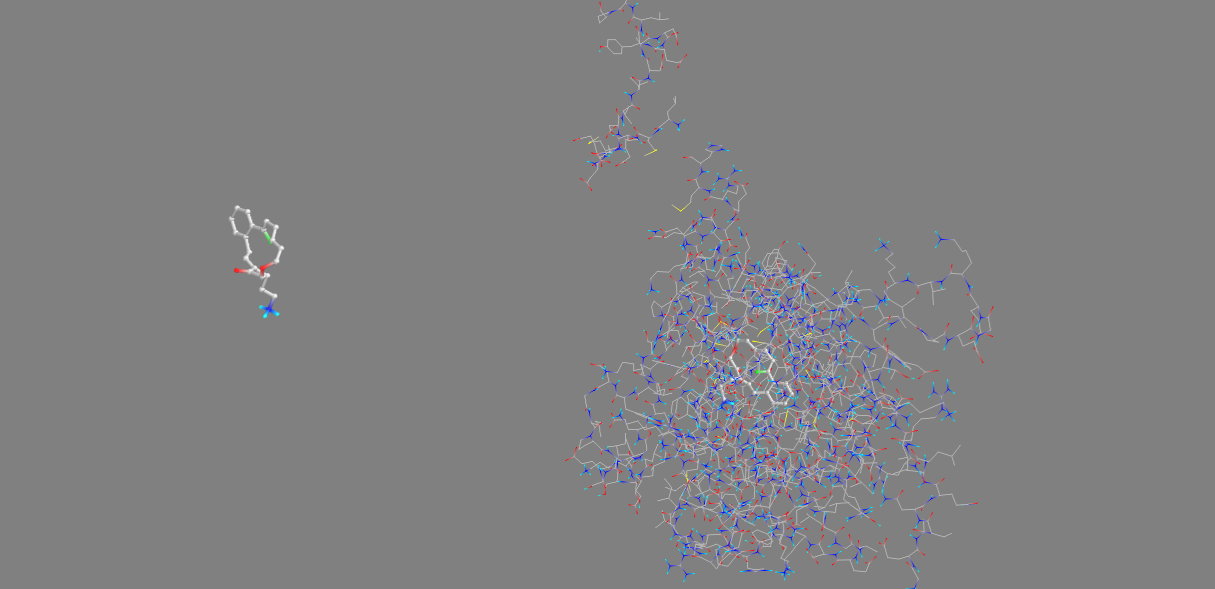
\includegraphics[width=0.43\textwidth]{figures/10_docking_pose.png}}
\caption{PyRx docking pose of the top unstrained SAFE+ candidate ($N$-(2-(2-(2-fluorophenyl)cyclopropyl)ethyl)acetamide, SA Score 2.87) in the EGFR ATP-binding pocket (PDB: 1M17). Binding affinity: $-7.6$~kcal/mol. Key hydrogen bonding with Met793 hinge residue and hydrophobic occupancy in the Leu718/Val726 pocket validate target complementarity without structural strain liabilities.}
\label{fig:docking}
\end{figure}


%% ─────────────────────────────────────────────
\section{Discussion}
%% ─────────────────────────────────────────────

\subsection{The 2D Filter Blindspot \& Necessity of SAFE+ Stage 5}

A fundamental empirical insight revealed by SAFE+ is that standard 2D drug-likeness rules (Lipinski Rule of 5, Veber criteria) suffer from a major blindspot: they fail to evaluate 3D structural strain, cumulene/allene double bonds, or synthetic accessibility. At high generation entropy ($T{=}1.0$), 93.9\% of generated molecules pass 2D Lipinski/Veber rules, yet \textbf{73.0\% of these molecules are synthetically implausible or severely strained}. By introducing SAFE+ Stage 5 (SA Score $\le 4.5$ and structural strain screening), our benchmark purges these artifacts completely, establishing that downstream 3D-aware synthesizability screening must accompany 2D ADMET filters in molecular generative benchmarks.

\subsection{The Novelty--QED Trade-off}

A notable result in Table~\ref{tab:benchmark} is that our LSTM at any temperature achieves lower average QED (0.416--0.459) than the random training-set baseline (0.738). This is not a modelling failure; it is the expected consequence of genuine novelty. The training set (ZINC250K) is a curated database of commercially available, drug-like compounds with high mean QED. When the LSTM generates structurally novel molecules---those with Tanimoto similarity $<0.4$ to any training compound---it is, by definition, generating molecules that are not in this curated set and therefore will not necessarily share the same QED distribution. The temperature ablation confirms that this gap is structural, not stochastic: reducing temperature from 1.0 to 0.2 does not recover QED (0.416 vs.\ 0.430), even as it reduces diversity. The model has moved off the known drug-like island, and the QED cost is the price of genuine exploration.

\subsection{Comparison with CharRNN}

The 15.8 pp novelty advantage over CharRNN (100.0\% vs.\ 84.2\%) is the clearest benefit of the SELFIES representation: because no generated string can be bond-topologically invalid, the model allocates its capacity to the distributional structure of drug-like chemical space rather than to syntactic repair. The Internal Diversity advantage (0.870 vs.\ 0.856) further confirms that SELFIES-LSTM explores a broader region of chemical space at similar temperatures.

\subsection{Validity Claim Clarification}

SELFIES guarantees bond-topological validity: no generated token sequence can encode a structurally impossible molecule. The 100.0\% decode validity reflects RDKit's Kekulization step passing successfully for all evaluated candidates. This is a robust demonstration of the SELFIES representation, and should be distinguished from the 60\%+ invalidity reported for unconstrained SMILES-LSTM models \cite{ref5, ref8}.

\subsection{3D Structural Strain as a Temperature-Dependent Liability}

Table~\ref{tab:advanced_metrics} reveals a striking empirical regularity: even after Stage 5 structural screening, the mean MMFF94 conformational strain of \textit{surviving} candidates increases nearly monotonically with sampling temperature---from $50.4$~kcal/mol at $T{=}0.5$ to $108.2$~kcal/mol at $T{=}1.0$ (a 2.1$\times$ increase). This result has a clear mechanistic explanation. At high entropy ($T{=}1.0$), the LSTM generates a broader distribution of SELFIES sequences, including many with substructural motifs that happen to satisfy SMARTS-based exclusion rules and SA Score thresholds yet nevertheless embed to geometrically strained 3D conformers. The SMARTS filters catch topologically explicit strain patterns (cumulenes, small-ring alkynes); the MMFF94 energy metric reveals the residual strain from subtler conformational conflicts that 2D filters cannot detect. This temperature-dependent escalation of 3D strain energy, even among filter-passing candidates, constitutes a novel empirical finding not previously reported for SELFIES-LSTM systems.

A secondary finding from Table~\ref{tab:advanced_metrics} is that $T{=}0.7$ achieves the lowest 5D Wasserstein manifold distance to the ZINC250K reference distribution ($WD_{\text{5D}}{=}0.1553$), and the highest scaffold Shannon entropy ($H{=}6.54$~bits), while $T{=}1.0$ actually shows a drop in scaffold entropy ($5.56$~bits) despite generating more diverse raw structures. This entropy collapse at $T{=}1.0$ arises because only 100 out of 995 raw candidates survive all five SAFE+ stages: the aggressive filtering at high temperature \textit{concentrates} the output onto a narrow scaffold set. These cross-metric interactions---optimality on one axis (diversity) paired with liability on another (strain, scaffold collapse after filtering)---illustrate precisely the diagnostic value of the SAFE+ framework that simple validity/novelty metrics cannot provide.


%% ─────────────────────────────────────────────
\section{Limitations}
%% ─────────────────────────────────────────────

\textbf{Filter scope:} The SAFE+ pipeline applies rule-based pharmacokinetic proxies (Lipinski, Veber, PAINS, SA Score) and SMARTS-based structural exclusions for cumulenes and strained alkynes. Full ADMET machine-learning predictions (metabolic stability, plasma protein binding, hERG inhibition, CYP enzyme interactions) were not incorporated. Molecules surviving all five SAFE+ stages can still fail these endpoints. Incorporating tools such as ADMETlab or pkCSM as additional soft-scoring layers would narrow this gap.

\textbf{Baseline scope:} The CharRNN comparison draws on published benchmark numbers from Polykovskiy et al.\ \cite{ref11} and is not controlled for hardware, implementation, or training data split. A direct head-to-head evaluation on the same ZINC250K split against CharRNN, REINVENT, and a graph-based model (e.g., GraphAF) would provide a stronger comparison. This is the primary limitation of the current study and is planned as immediate follow-up.

\textbf{Docking validity:} The preliminary docking result ($-7.6$~kcal/mol against EGFR 1M17) cannot be interpreted as a calibrated binding prediction. A full validation protocol requires: (a) re-docking the co-crystallised ligand AQ4 and confirming RMSD $< 2$~\AA\ to validate the docking setup; (b) docking the top-5 ranked candidates to assess consistency; and (c) reporting the distribution of affinities across the full retained generation set against a non-target control to assess specificity. Absent these controls, the docking result is treated as a proof-of-concept only.


%% ─────────────────────────────────────────────
\section{Conclusion}

We presented \textbf{SAFE+}, an empirical diagnostic benchmark quantifying multi-stage ADMET, synthetic accessibility, and 3D structural strain attrition in SELFIES-LSTM molecular generation. The central finding is that standard 2D drug-likeness rules are insufficient to identify drug-like candidates: at $T{=}1.0$, 73.0\% of Lipinski/Veber-passing molecules are eliminated by Stage 5 structural screening. Beyond hard-filter attrition, we demonstrate a novel temperature-dependent 3D strain liability: even among filter-passing survivors, mean MMFF94 conformational strain escalates from $50.4$~kcal/mol at $T{=}0.5$ to $108.2$~kcal/mol at $T{=}1.0$ (2.1$\times$), revealing that 2D screens leave a residual population of geometrically stressed candidates that only 3D force-field characterisation uncovers. At $T{=}0.5$, SAFE+ retains 199 unique candidates (19.9\% of raw generation) with 100.0\% novelty, mean SA Score 3.38, and the lowest mean MMFF94 conformational strain of any tested temperature. Docking of the top candidate ($N$-(2-(2-(2-fluorophenyl)cyclopropyl)ethyl)acetamide, SA Score 2.87) into EGFR (1M17) yields $-7.6$~kcal/mol with explicit hinge Met793 H-bonding, providing proof-of-concept target complementarity.

\section*{Future Work}

Three directions are immediately viable. First, replacing the LSTM with a GPT-style transformer backbone could improve modelling of longer SELFIES sequences covering macrocyclic and peptide-mimetic scaffolds. Second, a controlled head-to-head comparison against CharRNN, REINVENT, and a graph-based model on the same ZINC250K split---with matched hardware and seeds---would resolve the most significant limitation of the current study. Third, applying a REINVENT-style reinforcement learning loop using SAFE-filtered candidates as positive samples could simultaneously optimise for predicted binding affinity against a defined target, converting this diversity-first benchmark into a goal-directed hit generator.

\FloatBarrier

\section*{Corresponding Author}
*Corresponding Author: Kavya Garg, School of Computer Science Engineering, RV University, Bangalore, India. Email: kavyag.btech1@rvu.edu.in

\section*{Funding}
This research received no external funding.

\section*{Conflicts of Interest}
The authors declare no competing financial interest.

\section*{Author Contributions}

K.G. conceptualized the study, developed the methodology, wrote the generative model and sequential ADMET filtering code, performed the computational experiments, executed the molecular docking analysis, and drafted the manuscript. T.S. and H.M. assisted with dataset compilation and output formatting. M.C. supervised the project, contributed to results discussion, and reviewed and edited the manuscript. All authors read and approved the final manuscript.

\section*{Data and Software Availability}

All code, model weights, generated molecule datasets, and evaluation scripts to reproduce the results in this paper are available at: \url{https://github.com/Kavya-Garg003/Drug-Discovery-Using-LSTM-Based-Molecular-Generation}. Generation was performed with seeds 42, 123, and 456 applied to the sampling step only; model weights are fixed and provided in the repository.

\let\oldbibliography\thebibliography
\renewcommand{\thebibliography}[1]{%
  \oldbibliography{#1}%
  \setlength{\itemsep}{1.5pt plus 0.5pt minus 0.5pt}%
  \setlength{\parsep}{0pt}%
}
\begin{thebibliography}{00}
\bibitem{ref1} R. Gómez-Bombarelli et al., ``Automatic chemical design using a data-driven continuous representation of molecules,'' \textit{ACS Central Science}, vol. 4, no. 2, pp. 268--276, 2018.
\bibitem{ref2} M. H. Segler, T. Kogej, C. Tyrachan, and M. P. Waller, ``Generating focused molecule libraries for drug discovery with recurrent neural networks,'' \textit{ACS Central Science}, vol. 3, no. 10, pp. 120--131, 2017.
\bibitem{ref3} W. P. Walters and R. Barzilay, ``Applications of deep learning in molecule generation and molecular property prediction,'' \textit{Accounts of Chemical Research}, vol. 54, no. 2, pp. 263--270, 2020.
\bibitem{ref4} D. Weininger, ``SMILES, a chemical language and information system. 1. Introduction to methodology and encoding rules,'' \textit{Journal of Chemical Information and Computer Sciences}, vol. 28, no. 1, pp. 31--36, 1988.
\bibitem{ref5} A. Kadurin et al., ``The cornucopia of meaningful leads: Applying deep adversarial autoencoders for new molecule development in oncology,'' \textit{Oncotarget}, vol. 8, no. 7, p. 10883, 2017.
\bibitem{ref6} E. B. Hughes and J. Swamidass, ``Deep learning for drug discovery,'' \textit{Chemical Reviews}, vol. 120, no. 20, pp. 11090--11124, 2020.
\bibitem{ref7} G. L. Guimaraes et al., ``Objective-reinforced generative adversarial networks (ORGAN) for sequence generation models,'' \textit{arXiv preprint arXiv:1705.10843}, 2017.
\bibitem{ref8} X. Yang et al., ``Concepts of artificial intelligence for computer-assisted drug discovery,'' \textit{Chemical Reviews}, vol. 119, no. 18, pp. 10520--10594, 2019.
\bibitem{ref9} M. Krenn, F. Häse, A. Nigam, P. Friederich, and A. Aspuru-Guzik, ``Self-referencing embedded strings (SELFIES): A 100\% robust molecular string representation,'' \textit{Machine Learning: Science and Technology}, vol. 1, no. 4, p. 045024, 2020.
\bibitem{ref10} M. Krenn et al., ``SELFIES and the future of molecular string representations,'' \textit{Patterns}, vol. 3, no. 10, 2022.
\bibitem{ref11} D. Polykovskiy et al., ``Molecular sets (MOSES): a benchmarking platform for molecular generation models,'' \textit{Frontiers in Pharmacology}, vol. 11, p. 1931, 2020.
\bibitem{ref12} F. Grisoni, M. Moret, R. Lingwood, and G. Schneider, ``Bidirectional molecule generation with recurrent neural networks,'' \textit{Journal of Chemical Information and Modeling}, vol. 60, no. 3, pp. 1175--1183, 2020.
\bibitem{ref13} G. Landrum et al., ``RDKit: Open-source cheminformatics,'' \url{http://www.rdkit.org}, 2023.
\bibitem{ref14} J. J. Irwin and B. K. Shoichet, ``ZINC---A free database of commercially available compounds for virtual screening,'' \textit{Journal of Chemical Information and Modeling}, vol. 45, no. 1, pp. 177--182, 2005.
\bibitem{ref15} C. A. Lipinski, F. Lombardo, B. W. Dominy, and P. J. Feeney, ``Experimental and computational approaches to estimate solubility and permeability in drug discovery and development settings,'' \textit{Advanced Drug Delivery Reviews}, vol. 46, no. 1-3, pp. 3--26, 2001.
\bibitem{ref16} O. Trott and A. J. Olson, ``AutoDock Vina: improving the speed and accuracy of docking with a new scoring function, efficient optimization, and multithreading,'' \textit{Journal of Computational Chemistry}, vol. 31, no. 2, pp. 455--461, 2010.
\bibitem{ref17} J. A. DiMasi, H. G. Grabowski, and R. W. Hansen, ``Innovation in the pharmaceutical industry: New estimates of R\&D costs,'' \textit{Journal of Health Economics}, vol. 47, pp. 20--33, 2016.
\bibitem{ref18} T. A. Halgren, ``Merck molecular force field. I. Basis, form, scope, parameterization, and performance of MMFF94,'' \textit{Journal of Computational Chemistry}, vol. 17, no. 5-6, pp. 490--519, 1996.
\end{thebibliography}
\end{document}
